%adpitub
\chapter{Abstände}
\begin{inhalt}
  Abstände zwischen
  \begin{itemize}
    \item Punkt-Punkt, Punkt-Gerade, Punkt-Ebene
    \item Gerade-Gerade, Gerade-Ebene
    \item Ebene-Ebene
  \end{itemize}
\end{inhalt}

Abstände zwischen Objekten im Raum schreibt man $d(\text{Ding}_1, \text{Ding}_2)$

\begin{bla}{Punkt - Punkt}
  Der Abstand zweier Punkte $P,Q$ ist die Länge des Vektors $\overrightarrow{PQ}$:
  \[
  d(P,Q)
  =
  \left| \overrightarrow{PQ} \right|
  =
  \left|\begin{pmatrix}
    q_1 - p_1 \\ q_2 - p_2 \\ q_3 - p_3
  \end{pmatrix}\right|
  =
  \sqrt{(q_1 - p_1)^2 + (q_2 - p_2)^2 + (q_3 - p_3)^2}
  \]
\end{bla}

\begin{bla}{Punkt - Gerade: Laufender Punkt}
  \[
  \text{g: }\ \vec{x} = \vec{p} + r * \vec{u}
  \]
  Der Abstand zwischen Punkt $P$ und der Geraden $g$ ergibt sich, indem man den Abstand zwischen $P$ und einem beliebigen Punkt $Q$ auf der Gerade ausrechnet.
  Setzt man also für $Q$ die Geradengleichung ein, hängt $\overrightarrow{PQ}$ noch von dem Parameter r ab.
  Jetzt sucht man den Vektor, der senkrecht auf dem Richtungsvektor $\vec{u}$ der Geraden steht, also
  \[
  \overrightarrow{PQ} * \vec{u} = 0
  \]
  Man findet ein $r$ als Lösung der Gleichung.
  Damit hat man den Punkt $Q$ mit dem kürzesten Abstand und errechnet dann $d(P,Q)$.
\end{bla}



\begin{bla}{Punkt - Gerade: Hilfsebene}
  %
  \begin{marginfigure}[0em]
    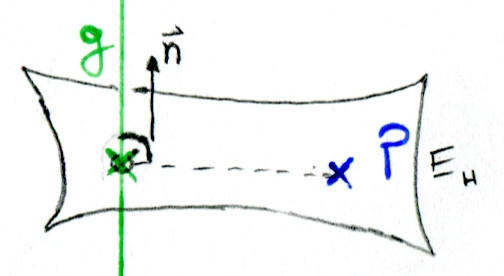
\includegraphics[scale=0.8]{AGAbstand_PktGerHilfsebene}
    \caption{Hilfsebene durch $P$, senkrecht zu Gerade g}
  \end{marginfigure}
  %
  Man baut sich eine Ebene E$_\text{H}$ senkrecht zu g, die durch $P$ geht:

  Damit die Gerade senkrecht auf der Ebene steht, wählt man als Normalenvektor $\vec{n}$ der Ebene den Richtungsvektor der Geraden $\vec{u}$.

  Damit die Ebene durch $P$ geht, wählt man $\vec{p}$ einfach als Stützvektor.

  Der Schnittpunkt zwischen Gerade und der neuen Ebene wird jetzt S genannt und kann einfach berechnet werden (siehe \ref{AG_LageGE}).

  Der Abstand vereinfacht sich zu:
  $d(P,g) = d(P,S)$
\end{bla}

\begin{bla}{Punkt - Ebene: Lotgerade}
  %
  \begin{marginfigure}[5em]
    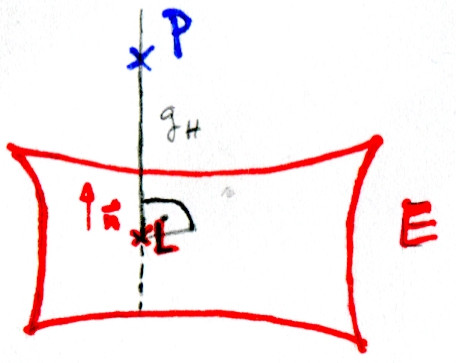
\includegraphics[scale=0.8]{AGAbstand_PktEbLotgerade}
    \caption{Lotgerade, senkrecht zur Ebene E, durch Punkt $P$}
  \end{marginfigure}
  %
  Man baut sich eine Gerade g$_\text{H}$, die durch P geht und senkrecht auf E steht:

  Als Stützvektor wählen wir $\vec{p}$, dann geht die Gerade durch P.

  Als Richtungsvektor wählen wir den Normalenvektor der Ebene: $\vec{n}$.

  Gesucht ist dann zuletzt der sogenannte \emph{Lotfußpunkt}: Der Schnittpunkt der Geraden mit der Ebene.
  Wir nennen ihn $L$ und finden ihn mit \ref{AG_LageGE}.

  Der Abstand vereinfacht sich dann auf zwei Punkte:
  $d(P,E) = d(P,L)$
\end{bla}

\begin{bla}{Punkt - Ebene: \textsc{Hesse}sche Normalenform}
  In der \textsc{Hesse}schen Normalenform kann der Punkt $P$ einfach auf der linken Seite der Gleichung eingesetzt werden, dann ergibt sich rechts der Abstand zur Ebene:
  \[
  \frac{ \left(n_1*x_1 + n_2*x_2 + n_3*x_3\right) - c}{|\vec{n}|}
  = d(P,E)
  \]
\end{bla}

\begin{bla}{Windschiefe Geraden: Laufende Punkte}
  Die beiden Geraden g und h sind windschief und wir suchen den Abstand:
  \begin{align*}
    \text{g: }\ \vec{x} = \vec{p} + r * \vec{u} \\
    \text{h: }\ \vec{x} = \vec{q} + s * \vec{v}
  \end{align*}
  Man nimmt zwei beliebige Punkte aus den Geradengleichungen und nennt sie zum Beispiel $G$ aus g und $H$ aus h.

  Deren Abstandsvektor $\overrightarrow{GH}$ hängt noch von $r$ und $s$ ab.
  Der kleinste Abstand ist der, bei dem $\overrightarrow{GH}$ auf beiden Richtungsvektoren $\vec{u}$ und $\vec{v}$ senkrecht steht:
  \begin{align*}
    \overrightarrow{GH} * \vec{u} = 0 \\
    \overrightarrow{GH} * \vec{v} = 0
  \end{align*}
  Dieses LGS hat zwei Gleichungen und liefert uns damit $r$ und $s$.

  Diese beiden setzen wir einfach in $\overrightarrow{GH}$ ein und haben den Abstandsvektor.
\end{bla}



\begin{bla}{Windschiefe Geraden: Hilfsebene}
  %
  \begin{marginfigure}[0em]
    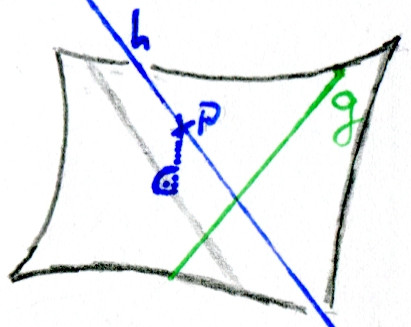
\includegraphics[scale=0.8]{AGAbstand_GerGerWindschief}
    \caption{Hilfsebene E, parallel zu beiden Geraden, g liegt in E}
  \end{marginfigure}
  %
  Die beiden Geraden g und h sind windschief und wir suchen den Abstand:
  \begin{align*}
    \text{g: }\ \vec{x} &= \vec{p} + r * \vec{u} \\
    \text{h: }\ \vec{x} &= \vec{q} + s * \vec{v}
    \intertext{Man konstruiert eine Ebene die parallel zu beiden Geraden liegt und die Gerade g sogar enthält:}
    \text{E}_\text{H} \text{: }\ \vec{x} &= \vec{p} + k * \vec{u} + l * \vec{v}
\end{align*}
  Die Gerade h hat zur ganzen Ebene den gleichen Abstand, also nimmt man einfach einen Punkt $P$ aus h und sucht den Abstand zur Ebene:
  \[
  d(\text{g},\text{h}) = d(P,\text{E})
  \]
\end{bla}

\begin{bla}{Parallele Geraden}
  Der Abstand ist entlang der gesamten Geraden gleich.
  Man nimmt aus einer Geraden einen beliebigen Punkt und berechnet den Abstand des Punktes zu der anderen Geraden.
\end{bla}

\begin{bla}{Gerade - Ebene}
  Abstände ergeben hier nur Sinn, wenn Gerade und Ebene parallel sind, weil sie sich sonst schneiden.

  Man sucht aus der Geraden einfach irgendeinen Punkt raus und rechnet dann den Abstand Punkt - Ebene.
\end{bla}

\begin{bla}{Ebene - Ebene}
  Abstände ergeben hier nur Sinn, wenn die Ebenen parallel sind, weil sie sich sonst schneiden.

  Man sucht aus einer der Ebenen einfach irgendeinen Punkt raus und rechnet dann den Abstand Punkt - Ebene.
\end{bla}
